\part*{第3章\\自己組織的チーム行動獲得システム}
\chapter{自己組織的チーム行動獲得システム}
\section{緒言}
ロボットやその頭脳としてのコンピュータの優れた能力は,繰り返し処理等のある決まった作業が容易に可能であることが挙げられる.しかし,状況い応じて変化する要素が含まれる際や,曖昧な情報を含有する際には,その処理能力は未だ人間には及ばない.ロボットに対して柔軟な処理の実装を試みる際には,生物の情報処理メカニズムからヒントを得た考え方,ソフトコンユーティング等の考え方が有効であると考えられている.\par
自律型ロボットの特徴を生かして大いに活用するためには,システムの管理運営について,効率化を重視し,中枢系を一つに集中する集中管理方式も好ましいが,各エージェント自体の自律性の向上が第一に望まれる.人間と試合可能なゴミ の実現のための課題には運動制御,環境認識,自己位置同定などが挙げられる.各エージェントとしてのロボットは得られたセンサ情報を基に,自身の状態の把握に加え,道徳性の同定を行い,環境の変化等も認識した上で,行動を決定することが望ましい.\par
サッカーロボットが環境を認識するためには,複数のセンサ情報から特徴を見つけ,状態や環境を認識するために必要な情報を抽出する必要がある.本節では自己組織化マップの低次元化及び汎化性能,特徴抽出能力に着目し,SOMを用いたサッカーロボットの環境認識から行動決定システムとして,サッカー試合中の人間による行動決定システムのロボットへの実装を提案する.


% =============================================
% セクション開始
%
% =============================================
\clearpage
\section{テンソル自己組織化マップ(TSOM)}
本論文ではニューラルネットワークの中でもテンソル自己組織化マップ(テンソルSOM)を用いて行動学習システム及び行動選択システムの開発を行う. テンソルSOMとはSOMをテンソルデータに拡張したものである. テンソルSOM のアルゴリズムを勝者決定, 近傍計算, モデルの更新の3つのステップにより簡潔に述べる.\cite{TSOM}(\ref{fig: tensor_shape}参照)

\begin{figure}[tbh]
 \centering
  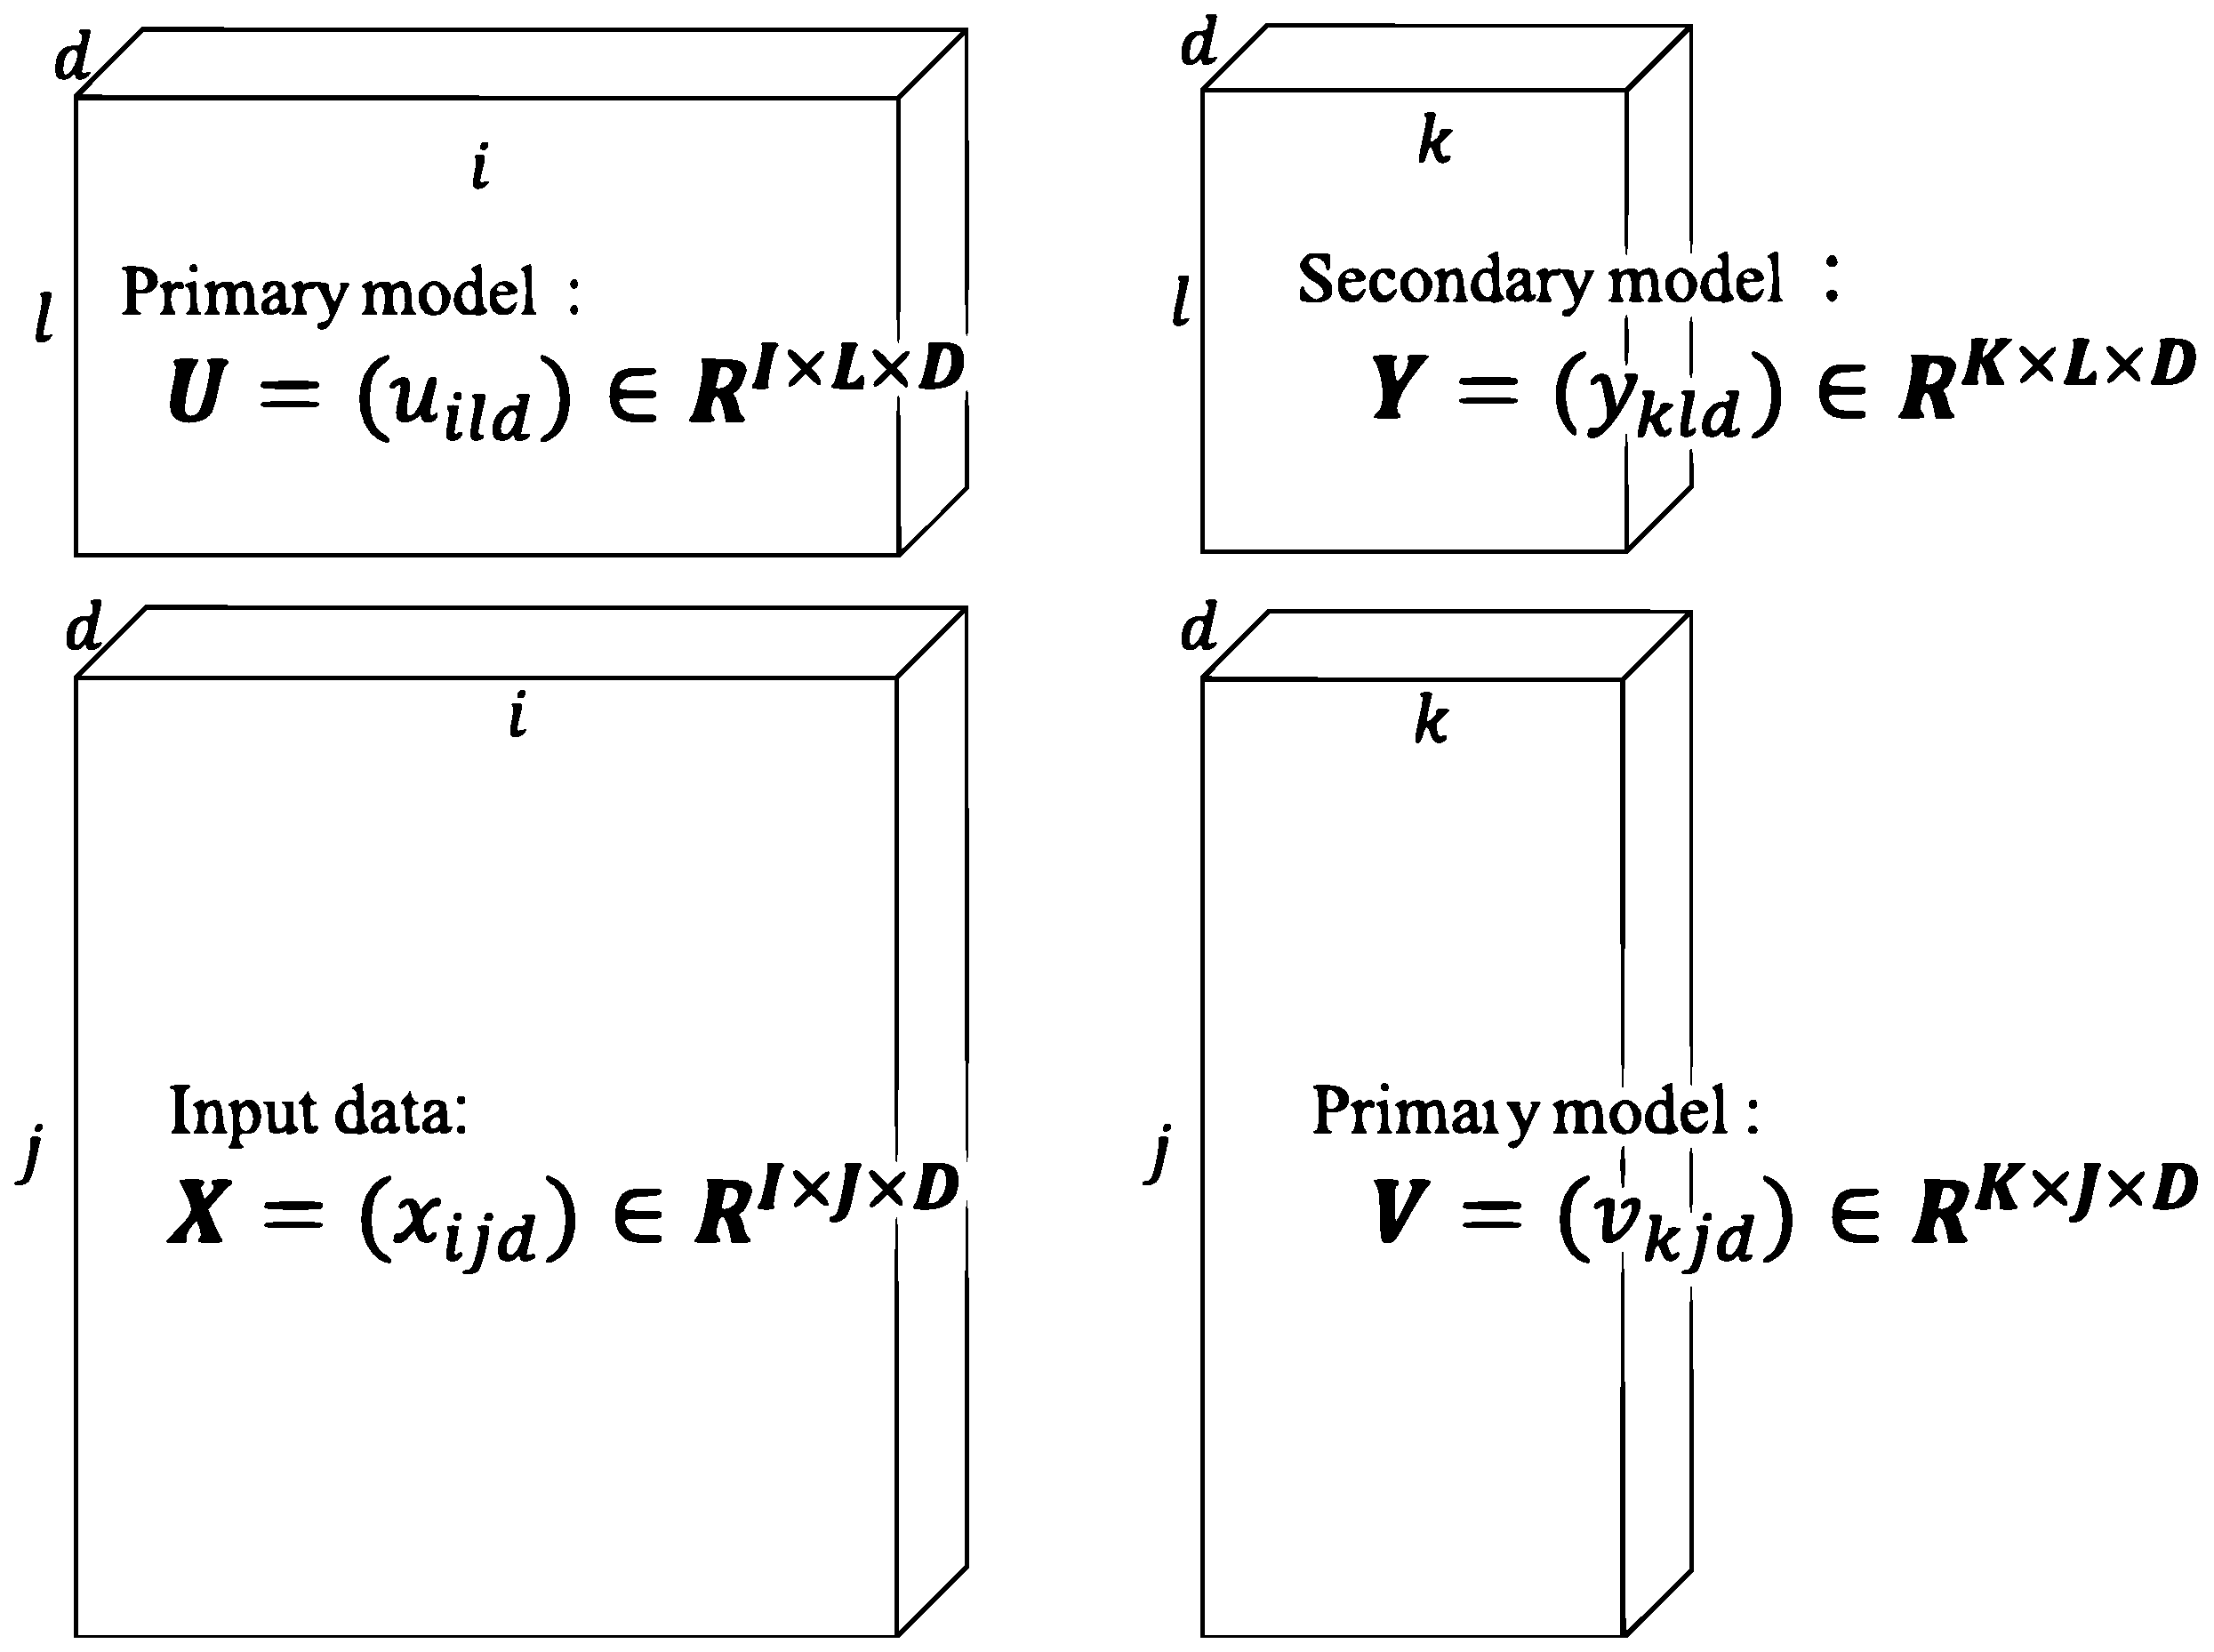
\includegraphics[clip,width=15.0cm]{figure/tensor_shape2.eps}
 % \vspace*{-4mm}
  \caption{Data image of tensor SOM}
  \label{fig: tensor_shape}
\end{figure}

\begin{enumerate}
	\item 勝者決定\\
	\ref{eqn: eq1},\ref{eqn: eq2}を用いて各モードの勝者(Best Matching Unit: BMU)を決定する. ここで$k_i^*$はモード1に対するBMU座標であり,$l_i^*$はモード2に対するBMU座標である.
	\begin{equation}
		k_{i^*} = \argmin_{k}\sum_{l=1}^L\sum_{d=1}^D{(u_{ild}-y_{kld})^2}
		\label{eqn: eq1}
	\end{equation}
	\begin{equation}
		l_j^* = \argmin_{l}\sum_{k=1}^K\sum_{d=1}^D{( v_{kjd}-y_{kld})^2}
		\label{eqn: eq2}
	\end{equation}
	
	\item 近傍計算\\
	 \ref{eqn: eq3},\ref{eqn: eq4}を用いて近傍を求める.$\alpha_{ki}$は, モード1に対するBMU近傍ユニットの変化量であり,$\beta_{lj}$も同様にモード2に関する変化量を示している.
	\begin{equation}
		\alpha_{ki}=\exp(-\frac{1}{2\sigma_{1}^2}\|\zeta_{k_i^*}^{(1)}-\zeta_k^{(1)}\|^2)
		\label{eqn: eq3}
	\end{equation}
	\begin{equation}
		\beta_{lj}=\exp(-\frac{1}{2\sigma_{2}^2}\|\zeta_{l_j^*}^{(2)}-\zeta_l^{(2)}\|^2)
		\label{eqn: eq4}
	\end{equation}
	
	\item モデルの更新\\
	\ref{eqn: eq5}~\ref{eqn: eq8}を用いて1次モデル,2次モデルともに更新する.
	\begin{itemize}
	\item 2次モデルの更新\\
	\begin{equation}
		y_{kld} = \frac{1}{g_kg_l}\sum_{i=1}^I\sum_{j=1}^J{\alpha_{ki}\beta_{lj}x_{ijd}}
		\label{eqn: eq5}
	\end{equation}
	\begin{equation}
	g_k = \sum_{i=1}^I{\alpha_{ki}}
		\label{eqn: eq6}
	\end{equation}
	\begin{equation}
	g_l = \sum_{j=1}^J{\beta_{lj}}
		\label{eqn: eq7}
	\end{equation}
	\item 1次モデルの更新\\
	\begin{equation}
	u_{ild} = \frac{1}{g_l}\sum_{j=1}^J{\beta_{lj}x_{ijd}}
		\label{eqn: eq8}
	\end{equation}
	\begin{equation}
	v_{kjd} = \frac{1}{g_k}\sum_{i=1}^I{\alpha_{ki}x_{ijd}}
		\label{eqn: eq9}
	\end{equation}
	\end{itemize}
	この3ステップを近傍半径である$\sigma$を時定数$\tau$に従って単調に減少させながら繰り返し行う.
\end{enumerate}

% =============================================
% セクション開始
%
% =============================================
\clearpage
\section{TSOMを用いた学習方法検証}
環境情報とそのときの取るべく望ましい行動は一種の入出力関係にある.このような入出力関係のある対の情報を一つのベクトルとして,TSOMへ入力することでその関係を得ることが可能である.ここでは,検証実験として,三次元空間のある平面状にある点の座標値を学習させ,$x$及び$y$の座標値から$z$の座標値を推定する実験を行った.
% =============================================
% セクション開始
%
% =============================================
\clearpage
\section{TSOMを用いた環境認識と行動決定}

% =============================================
% セクション開始
%
% =============================================
\clearpage
\section{人間と同じ行動判断アルゴリズムの創発}

人間と同じ行動決定創発を書き書きします

